
%% Report by Nithin M (13D070058)

\documentclass[11pt]{article}
\usepackage{amsmath}
\usepackage{amssymb}
\usepackage{amsthm}
\usepackage{graphicx}
\usepackage{float}
\usepackage{hyperref}
\usepackage{hyperref}

%\newtheorem*{defn}{Definition}

\title{RLC circuit}
\author{Nithin M (13D070058) }
\date{\today}
\begin{document}
\maketitle

\section{Introduction}
An RLC circuit is an electrical circuit consisting of a resistor (R), an inductor (L), and a capacitor (C), connected in series or in parallel. 

The program generates all the plots required for shown in this pdf and also the animation. You can find the full source code at \url{https://github.com/nithinmurali/acad_assignments}

\subsection{Versions required}
\begin{itemize}
\item pthon 2.7
\item jupyter 4.1.0
\item latex 3.14
\item Make 3.81
\end{itemize}



\section{Circuit Analysics}
\begin{figure}[H]
	\begin{center}
	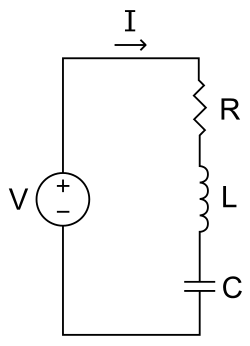
\includegraphics[scale=0.5]{source/RLC_series_circuit.png}
	\caption{Series RLC circuit}
	\centering
	\end{center}
\end{figure}

In this circuit, the three components are all in series with the voltage source. The governing differential equation can be found by substituting into Kirchhoff's voltage law (KVL) the constitutive equation for each of the three elements. 
\hfil \break
From the KVL, 
\begin{eqnarray*}
V_R + V_L + V_C = V(t) \\
V_R = RI(t) \\
V_L = L\frac{di}{dt} \\
V_C = \frac{1}{C}\int_{-\infty}^t I(\tau)\, d\tau = V(t)\
\end{eqnarray*}

For the case where the source is an unchanging voltage, differentiating and dividing by {{mvar|L}} leads to the second order differential equation:
\begin{equation}
\frac{d^2}{dt^2}I(t) + \frac{R}{L} \frac{d}{dt}I(t) + \frac{1}{LC} I(t) = 0
\label{eom}
\end{equation}

LC tank equation can usefully be expressed in a more generally applicable form:
\begin{equation}
\frac{d^2}{dt^2}I(t) + 2 \alpha \frac{d}{dt}I(t) + \omega_0^2 I(t) = 0
\label{diff_eqn}
\end{equation}

For the case of the series RLC circuit these two parameters are given by:
\begin{eqnarray}
\alpha = \frac{R}{2L} \\
\label{def_zeta}
\omega_0 = \frac{1}{\sqrt{LC}}
\label{def_omega}
\end{eqnarray}

A useful parameter is the damping factor, ζ, which is defined as the ratio of these two. In the case of the series RLC circuit, the damping factor is given by,
\begin{equation}
\zeta = \frac{R}{2} \sqrt\frac{C}{L}
\label{damp_fac}
\end{equation}


\section{Transient response}

The differential equation for the circuit solves in three different ways depending on the value of ζ,

\begin{itemize}
	\item{Under-damped system ($\zeta < 1$)}
	\item{Critically damped system ($\zeta = 1$)}
	\item{Over-damped system ($\zeta > 1$)}
	\item{Special Case ($\alpha = 0$)}
\end{itemize}

\newpage
\noindent\textbf{Under-damped system :} \\
In under-damped system $\zeta$ is less than 1. \\
The Response of the system is shown in the figure below.

\begin{equation}
I(t) = B e^{-\alpha t} \sin (\omega_\mathrm{d} t + \varphi)
\label{under-damped-eqn}
\end{equation}


\begin{figure}[H]
	\centering
	\centering
	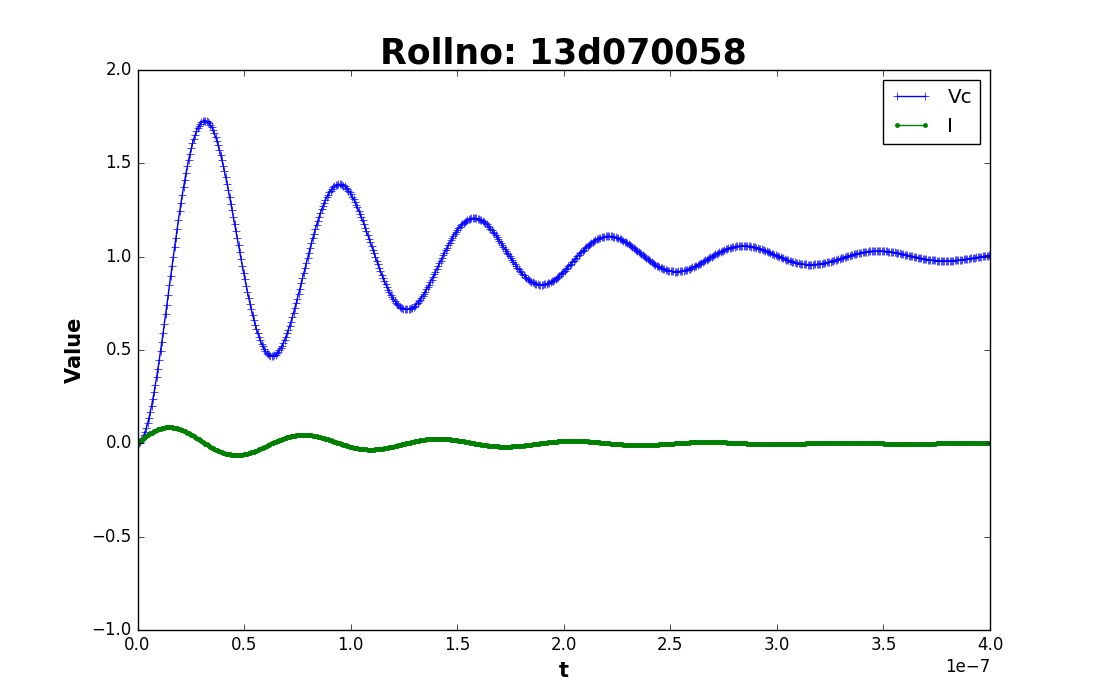
\includegraphics[scale=0.5]{output/underdamped.png}
	\caption{Response of the under damped series RLC system}
\end{figure}
\label{fig1}

\newpage
\noindent\textbf{Critically-damped system :} \\
In critically-damped system $\zeta$ is 1.
\begin{equation}
I(t) = D_1 t e^{-\alpha t} + D_2 e^{-\alpha t}
\label{critically-damped-eqn}
\end{equation}


The response of the system is shown in the figure below.

\begin{figure}[H]
	\centering
	\centering
	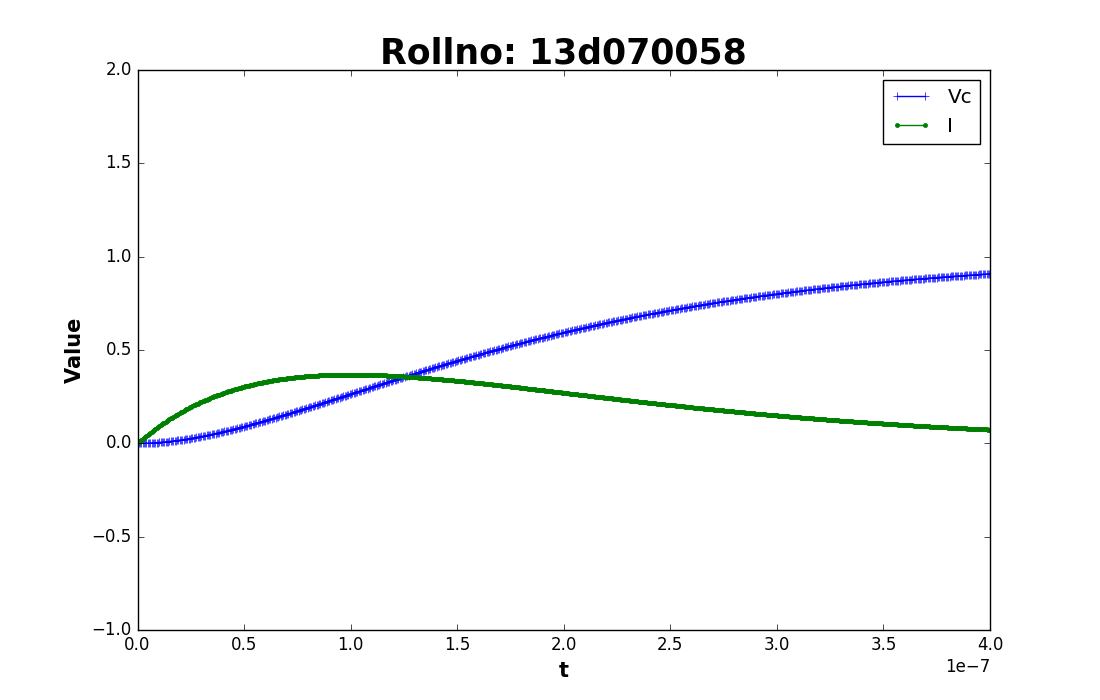
\includegraphics[scale=0.5]{output/criticallydamped.png}
	\caption{Response of the critically damped series RLC system}
\end{figure}
\label{fig2}

\newpage
\noindent\textbf{Over-damped system :} \\
In under-damped system $\zeta$ is more than 1.

\begin{equation}
I(t) = A_1 e^{-\omega_0 \left ( \zeta + \sqrt {\zeta^2 - 1} \right ) t} + A_2 e^{-\omega_0 \left ( \zeta - \sqrt {\zeta^2 - 1} \right ) t}
\label{critically-damped-eqn}
\end{equation}


The response of the system is shown in the figure below.

\begin{figure}[H]
	\centering
	\centering
	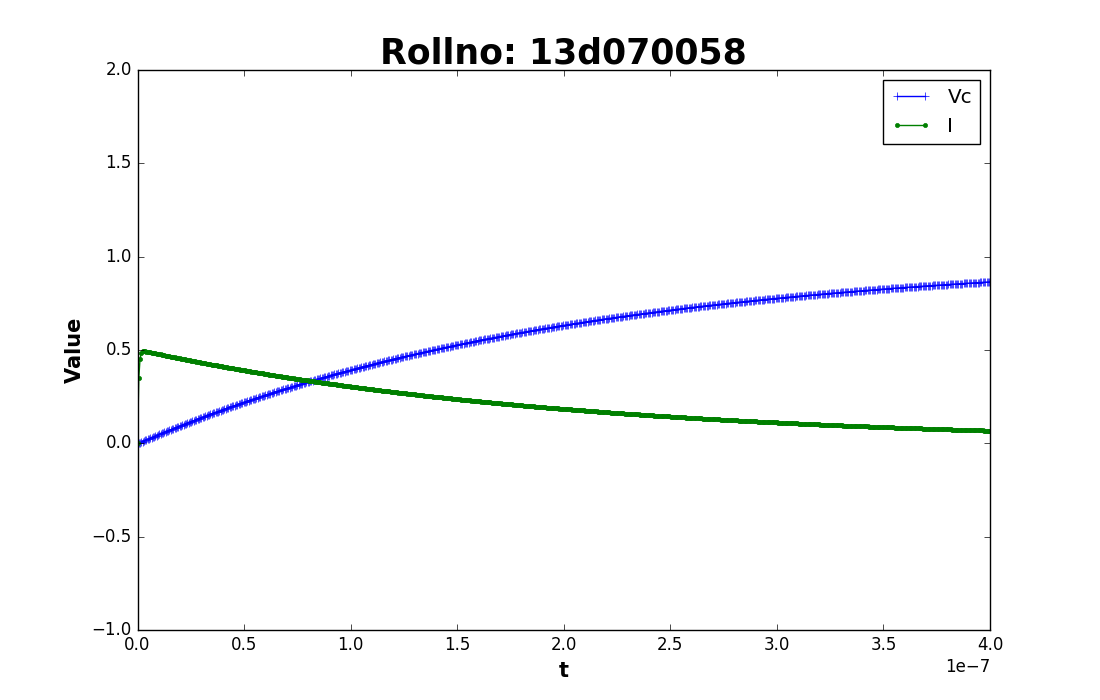
\includegraphics[scale=0.5]{output/overdamped.png}
	\caption{Response of the over damped series RLC system}
\end{figure}
\label{fig3}

\newpage
\noindent\textbf{Special case :} \\
A special case of the system arises when there is zero damping i.e $c = 0$ or $\zeta$ is zero. \\

The response of the system is shown in the figure below.

\begin{figure}[H]
	\centering
	\centering
	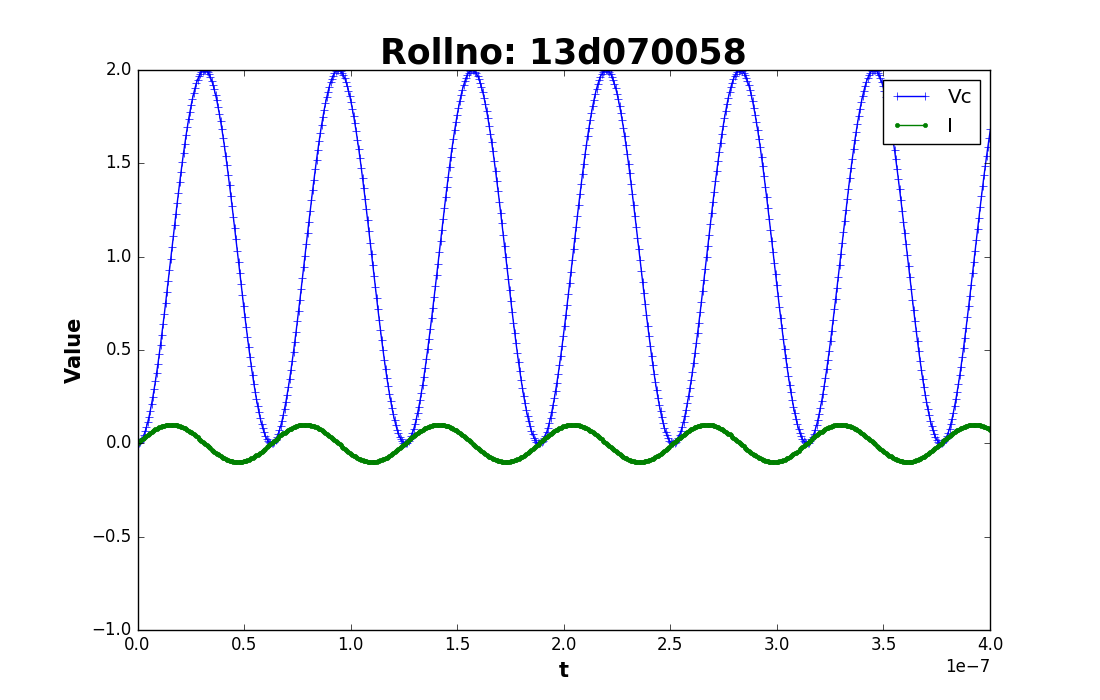
\includegraphics[scale=0.5]{output/special.png}
	\caption{Response of a special case}
\end{figure}
\label{fig4}

\section{Animation}

The below animation shows Capacitor voltage phasor in underdamped case. The animaiton is stored as 13d070058\_anim.mp4 in output folder.
\href{run:13d070058_anim.mp4}{play video}

\nocite{*}
\bibliography{bib_file}{}
\bibliographystyle{plain}
 
\end{document}